
\begin{figure}[!ht]
	\centering
	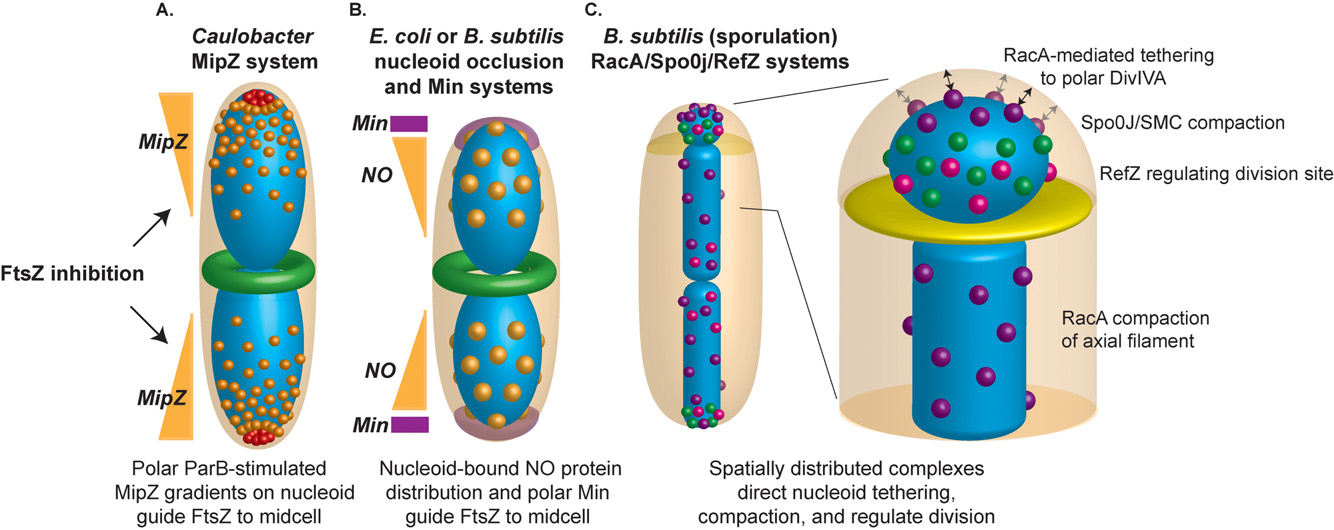
\includegraphics[width=0.9\linewidth]{figure/cytokinesis}
	\caption{Location of the FtsZ ring could be mediated by Nucleoid Occlusion (NO) molecules. These proteins bind on the first two thirds of the chromosome (depleted in the \textit{ter} region) and inhibit FtsZ polymerization. As long as segregation has not started, NO molecules inhibit FtsZ polymerization. Once chromosomes have migrated and the center of the cell only contains the unreplicated \textit{ter} region, FtsZ polymerization and septum formation start. Figure from \citet{ptacin_chromosome_2013}}
	\label{fig:cytokinesis}
\end{figure}

\textcolor[rgb]{1.00,0.00,0.00}{Depending on how it is modeled. The part on geometry is 'simple' to model:
\begin{itemize}
  \item volume division;
  \item changing the characteristics of the concerned volumes to adjust the surface of exchange for example.
\end{itemize}
Other part? Needs to be a cell process.}